\documentclass{article}

\usepackage[utf8]{inputenc}

\usepackage[top=2cm, bottom=3.5cm, left=2.5cm, right=2.5cm]{geometry}

\usepackage{enumitem}
\usepackage{booktabs}
\usepackage[T1]{fontenc}
\usepackage{float}

\usepackage{graphicx}
\usepackage{epstopdf}

%
% The following macro is used to generate the header.
% Arguments are
% Course, Semester+Year, Homework number, Due Date, Student
%
\newcommand{\homework}[5]{
   \thispagestyle{plain}
   \newpage
   \noindent
   \begin{center}
   \framebox{
      \vbox{\vspace{2mm}
    \hbox to 6.28in { {\bf #1 \hfill #2} }
       \vspace{6mm}
       \hbox to 6.28in { {\Large \hfill Homework \##3 - Due date: #4\hfill} }
       \vspace{4mm}
       \hbox to 6.28in { {\hfill Student: #5} }
      \vspace{2mm}}
   }
   \end{center}
}

% Style of greek letters
\renewcommand{\phi}{\varphi}
\renewcommand{\epsilon}{\varepsilon}

\usepackage{titlesec}
\usepackage{sectsty}
\allsectionsfont{\mdseries\scshape}
\titlelabel{{\mdseries\scshape Problem }\thesection\ -\ }
\newcommand{\problem}{\section}

% Macros EPFL-MLO
\usepackage{amssymb,amsmath,amsthm,dsfont}

% Indicator function
\usepackage{bbm}
\providecommand{\ind}[1]{\mathbbm{1}_{\{#1\}}}

\providecommand{\lin}[1]{\ensuremath{\left\langle #1 \right\rangle}}
\providecommand{\abs}[1]{\ensuremath{\left\lvert#1\right\rvert}}
\providecommand{\norm}[1]{\ensuremath{\left\lVert#1\right\rVert}}

\providecommand{\refLE}[1]{\ensuremath{\stackrel{(\ref{#1})}{\leq}}}
\providecommand{\refEQ}[1]{\ensuremath{\stackrel{(\ref{#1})}{=}}}
\providecommand{\refGE}[1]{\ensuremath{\stackrel{(\ref{#1})}{\geq}}}
\providecommand{\refID}[1]{\ensuremath{\stackrel{(\ref{#1})}{\equiv}}}

  % basic sets
  \providecommand{\R}{\mathbb{R}} % Reals
  \providecommand{\N}{\mathbb{N}} % Naturals
  
  % random variables
  \DeclareMathOperator{\E}{{\mathbb E}}
  %\providecommand{\E}[1]{{\mathbb E}\left.#1\right. }     %expectation
  \providecommand{\Eb}[1]{\ensuremath{\E \left[#1\right] }} %expectation, with brackets
  \providecommand{\EE}[2]{\E_{#1} \! #2 }      %expectation  
  \providecommand{\EEb}[2]{\ensuremath{\E_{#1}\!\! \left[#2\right] }} %expectation,  with brackets
  \providecommand{\prob}[1]{\ensuremath{{\rm Pr}\left[#1\right] } }
  \providecommand{\Prob}[2]{\ensuremath{{\rm Pr}_{#1}\left[#2\right] } }
  \providecommand{\P}[1]{\ensuremath{{\rm Pr}\left.#1\right. }}
  \providecommand{\Pb}[1]{\ensuremath{{\rm Pr}\left[#1\right] }}
  \providecommand{\PP}[2]{\ensuremath{{\rm Pr}_{#1}\left[#2\right] }}
  \providecommand{\PPb}[2]{\ensuremath{{\rm Pr}_{#1}\left[#2\right] }}
  
  \newcommand\independent{\protect\mathpalette{\protect\independenT}{\perp}}
  \def\independenT#1#2{\mathrel{\rlap{$#1#2$}\mkern2mu{#1#2}}}

  % operators
  \DeclareMathOperator*{\argmin}{arg\,min}
  \DeclareMathOperator*{\argmax}{arg\,max}
  \DeclareMathOperator*{\supp}{supp}
  \DeclareMathOperator*{\diag}{diag}
  \DeclareMathOperator*{\Tr}{Tr}
  
  % bold vectors
  \providecommand{\0}{\mathbf{0}}
  \providecommand{\1}{\mathbf{1}}
  \renewcommand{\aa}{\mathbf{a}}
  \providecommand{\bb}{\mathbf{b}}
  \providecommand{\cc}{\mathbf{c}}
  \providecommand{\dd}{\mathbf{d}}
  \providecommand{\ee}{\mathbf{e}}
  \providecommand{\ff}{\mathbf{f}}
  \let\ggg\gg
  \renewcommand{\gg}{\mathbf{g}}
  \providecommand{\gv}{\mathbf{g}}
  \providecommand{\hh}{\mathbf{h}}
  \providecommand{\ii}{\mathbf{i}}
  \providecommand{\jj}{\mathbf{j}}
  \providecommand{\kk}{\mathbf{k}}
  \let\lll\ll
  \renewcommand{\ll}{\mathbf{l}}
  \providecommand{\mm}{\mathbf{m}}
  \providecommand{\nn}{\mathbf{n}}
  \providecommand{\oo}{\mathbf{o}}
  \providecommand{\pp}{\mathbf{p}}
  \providecommand{\qq}{\mathbf{q}}
  \providecommand{\rr}{\mathbf{r}}
  \renewcommand{\ss}{\mathbf{s}}
  \providecommand{\tt}{\mathbf{t}}
  \providecommand{\uu}{\mathbf{u}}
  \providecommand{\vv}{\mathbf{v}}
  \providecommand{\ww}{\mathbf{w}}
  \providecommand{\xx}{\mathbf{x}}
  \providecommand{\yy}{\mathbf{y}}
  \providecommand{\zz}{\mathbf{z}}
  
  % bold matrices
  \providecommand{\mA}{\mathbf{A}}
  \providecommand{\mB}{\mathbf{B}}
  \providecommand{\mC}{\mathbf{C}}
  \providecommand{\mD}{\mathbf{D}}
  \providecommand{\mE}{\mathbf{E}}
  \providecommand{\mF}{\mathbf{F}}
  \providecommand{\mG}{\mathbf{G}}
  \providecommand{\mH}{\mathbf{H}}
  \providecommand{\mI}{\mathbf{I}}
  \providecommand{\mJ}{\mathbf{J}}
  \providecommand{\mK}{\mathbf{K}}
  \providecommand{\mL}{\mathbf{L}}
  \providecommand{\mM}{\mathbf{M}}
  \providecommand{\mN}{\mathbf{N}}
  \providecommand{\mO}{\mathbf{O}}
  \providecommand{\mP}{\mathbf{P}}
  \providecommand{\mQ}{\mathbf{Q}}
  \providecommand{\mR}{\mathbf{R}}
  \providecommand{\mS}{\mathbf{S}}
  \providecommand{\mT}{\mathbf{T}}
  \providecommand{\mU}{\mathbf{U}}
  \providecommand{\mV}{\mathbf{V}}
  \providecommand{\mW}{\mathbf{W}}
  \providecommand{\mX}{\mathbf{X}}
  \providecommand{\mY}{\mathbf{Y}}
  \providecommand{\mZ}{\mathbf{Z}}
  \providecommand{\mLambda}{\mathbf{\Lambda}}
  
  % caligraphic
  \providecommand{\cA}{\mathcal{A}}
  \providecommand{\cB}{\mathcal{B}}
  \providecommand{\cC}{\mathcal{C}}
  \providecommand{\cD}{\mathcal{D}}
  \providecommand{\cE}{\mathcal{E}}
  \providecommand{\cF}{\mathcal{F}}
  \providecommand{\cG}{\mathcal{G}}
  \providecommand{\cH}{\mathcal{H}}
  \providecommand{\cI}{\mathcal{I}}
  \providecommand{\cJ}{\mathcal{J}}
  \providecommand{\cK}{\mathcal{K}}
  \providecommand{\cL}{\mathcal{L}}
  \providecommand{\cM}{\mathcal{M}}
  \providecommand{\cN}{\mathcal{N}}
  \providecommand{\cO}{\mathcal{O}}
  \providecommand{\cP}{\mathcal{P}}
  \providecommand{\cQ}{\mathcal{Q}}
  \providecommand{\cR}{\mathcal{R}}
  \providecommand{\cS}{\mathcal{S}}
  \providecommand{\cT}{\mathcal{T}}
  \providecommand{\cU}{\mathcal{U}}
  \providecommand{\cV}{\mathcal{V}}
  \providecommand{\cX}{\mathcal{X}}
  \providecommand{\cY}{\mathcal{Y}}
  \providecommand{\cW}{\mathcal{W}}
  \providecommand{\cZ}{\mathcal{Z}}

% Commenting
\RequirePackage[colorinlistoftodos,bordercolor=orange,backgroundcolor=orange!20,linecolor=orange,textsize=scriptsize]{todonotes}
\providecommand{\comment}[2]{\todo[inline,caption={}]{\textbf{#1: }#2}}%
\providecommand{\inlinecomment}[3]{%
  %\@getnewcolor%
  %\edef\@tempa{\@colstring}%
  {\color{#1}#2: #3}}%
\newcommand\commenter[2]%
{%
  \expandafter\newcommand\csname i#1\endcsname[1]{\inlinecomment{#2}{#1}{##1}}
  \expandafter\newcommand\csname #1\endcsname[1]{\comment{#1}{##1}}
}

% Use these for theorems, lemmas, proofs, etc.
\newtheorem{proposition}{Proposition}
\newtheorem{lemma}{Lemma}
\newtheorem{corollary}[lemma]{Corollary}
%\newtheorem{conjecture}[lemma]{Conjecture}
\newtheorem{definition}{Definition}
\newtheorem{remark}[lemma]{Remark}
\newtheorem{assumption}{Assumption}
\newtheorem{theorem}[lemma]{Theorem}
\newtheorem{example}[lemma]{Example}

\newtheorem{claim}{Claim}
\newtheorem{fact}{Fact}

\definecolor{mydarkblue}{rgb}{0,0.08,0.45}
\usepackage[colorlinks=true,linkcolor=blue]{hyperref} 
\hypersetup{ %
    colorlinks=true,
    linkcolor=mydarkblue,
    citecolor=mydarkblue,
    filecolor=mydarkblue,
    urlcolor=mydarkblue
}
\usepackage[capitalize,noabbrev]{cleveref}


\usepackage{url}
\def\UrlBreaks{\do\/\do-}

\usepackage[round]{natbib}
\renewcommand{\cite}[1]{\citep{#1}}



\makeatletter
\newcommand{\skipitems}[1]{%
  \addtocounter{\@enumctr}{#1}%
}
\makeatother

\begin{document}
    \homework{COM-514: Mathematical Foundations of Signal Processing}{Fall 2019}{3}{20\textsuperscript{th} December 2019}{Oriol Barbany Mayor}
    
    \problem{Maximum SNR Beamformer}
    Let $R_z$ be the covariance matrix of the signal and $R_e$ the covariance matrix of the noise. Given that both are zero-mean WSS,
    \begin{align}
        \text{SNR}=\frac{\E[|\hh^* z_n|^2]}{\E[|\hh^* e_n|^2]}=\frac{\hh^* R_z \hh}{\hh^* R_e \hh}
    \end{align}
    
    To find the maximum, equate the gradient to zero. Given that any covariance matrix is self-adjoint,
    \begin{align}
        \nabla_{\hh}\text{SNR}=\frac{2R_z \hh \hh^* R_e \hh - 2 \hh^* R_z \hh R_e \hh}{(\hh^* R_e \hh)^2}=0
    \end{align}
    
    Given that $R_e \succ 0$, we can invert this matrix and we get the generalized eigenvalue problem.
    \begin{align}
        R_z \hh = \frac{\hh^* R_z \hh}{\hh^* R_e \hh}R_e \hh \Longrightarrow R_e^{-1}R_z \hh = \frac{\hh^* R_z \hh}{\hh^* R_e \hh}\hh
    \end{align}
    
    Now, given that $z_n=\aa(\theta)s_n$ and $s_n$ is a narrow-band zero-mean WSS signal, $R_z=\sigma_s^2 \aa(\theta)\aa^*(\theta)$. Substituting into the latter expression, we get
    \begin{align}
        \sigma_s^2 R_e^{-1} \aa(\theta)\aa^*(\theta)\hh = \sigma_s^2 \frac{\hh^* \aa(\theta)\aa^*(\theta) \hh}{\hh^* R_e \hh}\hh
    \end{align}
    
    Rearranging terms, we get the desired result
    \begin{align}
        R_e^{-1} \aa(\theta) = \frac{\hh^* \aa(\theta)}{\hh^* R_e \hh}\hh \Longrightarrow \hh = \frac{\hh^* R_e \hh}{\hh^* \aa(\theta)}R_e^{-1} \aa(\theta)
        \end{align}
    
    \problem{Splines (I)}
    \begin{enumerate}[label=(\roman*)]
        \item To find the values $a_1,a_2$ it's enough to impose the boundary conditions
        \begin{align}
            s_1(1)=a_1 = f(1)=\frac{1}{1} \Longrightarrow a_1 = 1 \qquad ; \qquad s_2(4)=a_2=f(4)=\frac{1}{4} \Longrightarrow a_2 = \frac{1}{4}
        \end{align}
        \item The rows of the matrix correspond to the following constraints:
        \begin{enumerate}[label=\arabic*.]
            \item $s_1'(1)=f'(1)=\frac{-1}{1^2}$
            \item $s_1(4)=f(4)=\frac{1}{4}$
            \item $s_1'(4)=s_2'(4)$
            \item $s_1''(4)=s_2''(4)$
            \item $s_2(5)=f(5)=\frac{1}{5}$
             \item $s_2'(5)=f'(5)=\frac{-1}{5^2}$
        \end{enumerate}
        \begin{align}
            \begin{bmatrix}
            1 & 0 & 0 & 0 & 0 & 0 \\
            (4-1) & (4-1)^2 & (4-1)^3 & 0 & 0 & 0\\
             1 & 2(4-1) & 3(4-1)^2 & -1 & 0 & 0 \\
            0 & 2 & 6(4-1) & 0 & -2 & 0 \\
            0 & 0 & 0 & (5-4) & (5-4)^2 & (5-4)^3 \\
            0 & 0 & 0 & 1 & 2(5-4) & 3(5-4)^2 \\
            \end{bmatrix}
            \begin{bmatrix}
                b_1 \\
                c_1 \\
                d_1 \\
                b_2 \\
                c_2 \\
                d_2
            \end{bmatrix}
            =
            \begin{bmatrix}
                -1 \\
                \frac{1}{4} - a_1 \\
                0 \\
                0 \\
                \frac{1}{5}-a_2 \\
                -\frac{1}{25} \\
            \end{bmatrix}
        \end{align}
        
        Solving the previous linear system, gives the cubic spline approximation depicted in \autoref{fig:spline}.
        
        \begin{figure}
            \centering
            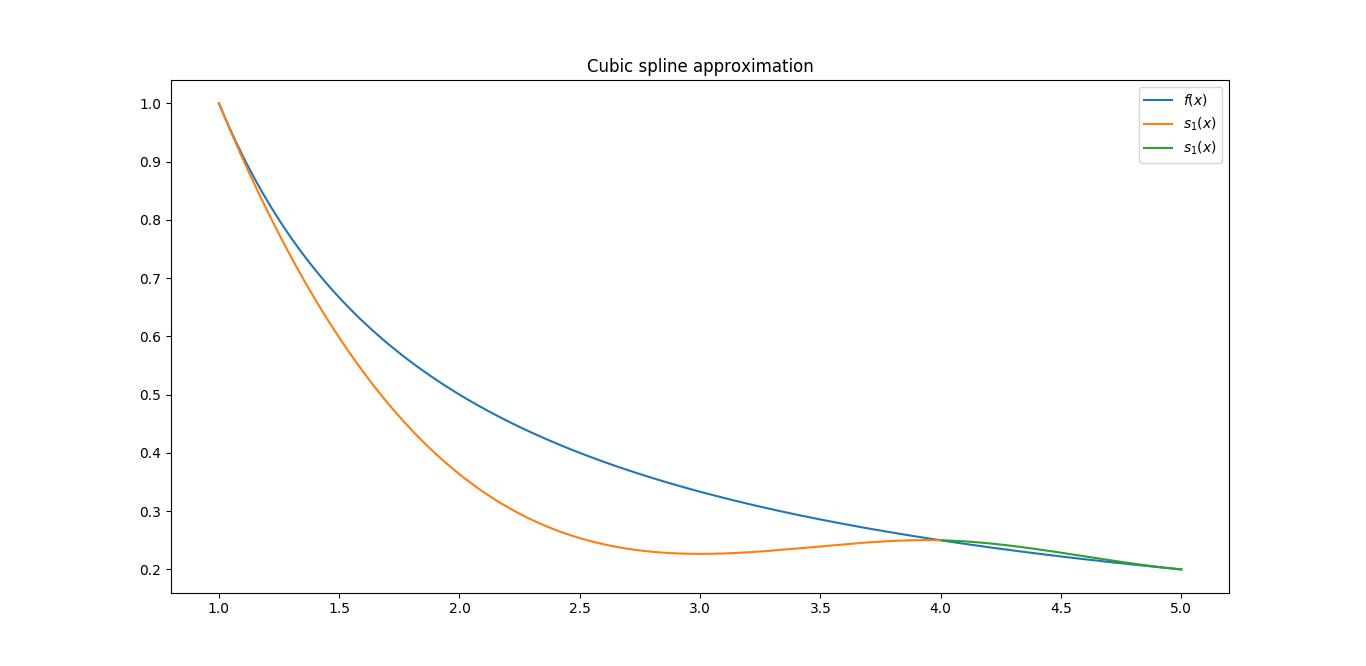
\includegraphics[width=.7\textwidth]{spline_app.png}
            \caption{Cubic spline approximation of $f(x)=\frac{1}{x}$ with clamped boundary conditions}
            \label{fig:spline}
        \end{figure}
        
        \item Let $d(x):=f(x)-s(x)$. Then, using integration by parts in each subinterval,
        \begin{align}
            \int_a^b s''(x)d''(x)dx&:=\int_a^b s''(x)(f''(x) - s''(x))dx\\
            &=\sum_{i=1}^{n-1}\int_{x_i}^{x_{i+1}} s''(x)(f''(x) - s''(x))dx \\
            &=\sum_{i=1}^{n-1} s''(x)(f'(x)-s'(x))\bigg\rvert_{x_i}^{x_{i+1}} - \int_{x_i}^{x_{i+1}}  s'''(x)(f'(x) - s'(x))dx
            \label{eq:subinterval}
        \end{align}
        
        The spline is chosen so that $f(x_i)=s(x_i) \ \forall i\in [1,2,\dots, n]$. Moreover, given that $s$ is a cubic Spline, the function $s'''$ is a constant, namely $c\in \mathbb{C}$. Hence, 
        \begin{align}
            \int_{x_i}^{x_{i+1}}  s'''(x)(f'(x) - s'(x))dx &= c \int_{x_i}^{x_{i+1}}(f'(x) - s'(x))dx \\
            &= c[f(x_i)-f(x_{i+1})-(s(x_i)-s(x_{i+1}))]=0
            \label{eq:const}
        \end{align}
        
        Mixing \eqref{eq:subinterval} and \eqref{eq:const} and telescoping,
        \begin{align}
            \int_a^b s''(x)d''(x)dx&:=\sum_{i=1}^{n-1} s''(x)(f'(x)-s'(x))\bigg\rvert_{x_i}^{x_{i+1}} \\
            &= \sum_{i=1}^{n-1} s''(x_{i+1})(f'(x_{i+1})-s'(x_{i+1})) - s''(x_{i})(f'(x_{i})-s'(x_i)) \\
            &=s''(b)(f'(b)-s'(b)) - s''(a)(f'(a)-s'(a)) =0
            \label{eq:0}
        \end{align}
        where the last equality follows by the clamped boundary conditions.
        
        \item Using \eqref{eq:0}, we have that
        \begin{align}
            \int_a^b s''(x)(s''(x) - f''(x)) dx = 0 \Longleftrightarrow \int_a^b [s''(x)]^2dx = \int_a^b s''(x) f''(x) dx
            \label{eq:equality}
        \end{align}
        
        Given the latter, we can write
        \begin{align}
           \int_{a}^b [f''(x)-s''(x)]^2 dx &=  \int_{a}^b [f''(x)]^2 dx -  2\int_{a}^b f''(x)s''(x)dx +  \int_{a}^b [s''(x)]^2 dx \\
           &\refEQ{eq:equality} \int_{a}^b [f''(x)]^2 dx -  2\int_{a}^b [s''(x)]^2 dx +  \int_{a}^b [s''(x)]^2 dx \\
           &=\int_{a}^b [f''(x)]^2 dx - \int_{a}^b [s''(x)]^2 dx \geq 0
        \end{align}
        where the last inequality follows since we are integrating a non-negative function. The proof concludes by rearranging these terms:
        \begin{align}
          \int_{a}^b [f''(x)]^2 dx \geq \int_{a}^b [s''(x)]^2 dx
        \end{align}
    \end{enumerate}
    \problem{Splines (II)}
    \begin{enumerate}
        \item The minimum value of $K$ would be 1, since the signal $x(t)$ is piece-wise linear.
        \item Let $x(t)=\sum_{k \in \mathbb{Z}}\alpha_k \beta_+^{(1)}(t-k)$. Given that the B-spline of degree 1 is defined as a triangle of height 1 from 0 to 1, and the signal $x(t)$ is piece-wise linear, it's easy to find the values of $\alpha_k$ graphically.
        \begin{align}
            \alpha = \begin{bmatrix}
                \cdots &
                0 &
                \fbox{1} &
                1 &
                3 &
                -1 &
                0 &
                \cdots
            \end{bmatrix}^T
            \label{eq:alpha}
        \end{align}
        \item Using Fubini's theorem,
        \begin{align}
            \int_{-\infty}^t x(\tau) d\tau &= \int_{-\infty}^t\sum_{k \in \mathbb{Z}}\alpha_k \beta_+^{(1)}(\tau-k) d\tau=\sum_{k \in \mathbb{Z}}\alpha_k \int_{-\infty}^t \beta_+^{(1)}(\tau-k) d\tau =\sum_{k \in \mathbb{Z}}\alpha_k \int_{-\infty}^{t-k} \beta_+^{(1)}(s) ds 
        \end{align}
        
        Given that the causal elementary B-spline of degree $K$ is defined as $\beta_+^{(K)}:=\beta_+^{(K-1)} \ast \beta_+^{(0)}$,
        \begin{align}
        \int_{-\infty}^t x(\tau) d\tau  &= \sum_{k \in \mathbb{Z}}\alpha_k \int_{-\infty}^{t-k} \beta_+^{(1)}(s) ds= \sum_{k \in \mathbb{Z}}\alpha_k \sum_{m=0}^{\infty}\int_{t-k-m-1}^{t-k-m} \beta_+^{(1)}(s) ds \\
        &=: \sum_{k \in \mathbb{Z}}\alpha_k\sum_{m=0}^{\infty}\int_{-\infty}^{\infty} \beta_+^{(1)}(s) \beta_+^{(0)}(t-k-m-s) ds \\
        &= \sum_{k \in \mathbb{Z}}\alpha_k\sum_{m=0}^{\infty} (\beta_+^{(1)} \ast  \beta_+^{(0)})((t-k-m)) 
        \\&=: \sum_{k \in \mathbb{Z}}\alpha_k\sum_{m=0}^{\infty} \beta_+^{(2)}(t-k-m) \\
        &=\sum_{k \in \mathbb{Z}}\alpha_k \sum_{n=k}^{\infty} \beta_+^{(2)}(t-n)=\sum_{n \in \mathbb{Z}} \left[\sum_{k=-\infty}^{n}\alpha_k \right] \beta_+^{(2)}(t-n) \\
        &=: \sum_{n \in \mathbb{Z}} b_n \beta_+^{(2)}(t-n)
        \end{align}
        
        So, using the latter and \eqref{eq:alpha}, we have that
        \begin{align}
            \alpha = \begin{bmatrix}
                \cdots &
                0 &
                \fbox{1} &
                2 &
                5 &
                4 &
                4 &
                \cdots
            \end{bmatrix}^T
        \end{align}
        
    \end{enumerate}
\end{document}

